\documentclass{scrartcl}
\usepackage[utf8]{inputenc}
\usepackage[english]{babel}
\usepackage{caption}
\usepackage{listings}
\usepackage{pdfpages}
\usepackage{amsmath,amssymb}

\newcommand{\qed}{\hfill $\blacksquare$}

\lstset{frame=single,keepspaces=true,captionpos=b}

\title{Homework 06 - Optimization}
\author{Arne Sachtler - \textit{Registration Number: 03692662}}
\date{\today}
\subtitle{IN2064 Machine Learning}

\begin{document}
\maketitle
	
\section{Convexity}
\subsection{Problem 1}
\begin{itemize}
	\item \textbf{i)}\\
	Given the function
	\begin{equation}
		f(x,y,z) = 3x + e^{y+z} - \min\{-x^2, \log(y)\} \text{ on } D = (-100,100)\times(1,50)\times(10,20)
	\end{equation}
	$f$ can be decomposed into a sum of three functions:
	\begin{equation}
		f(x,y,z) = g(x) + h(y,z) + k(x,y)\, ,
	\end{equation}
	where 
	\begin{enumerate}
		\item $g(x) = 3x$
		\item $h(y,z) = e^{y+z}$
		\item $k(x,y) = -\min(-x^2, \log(y))$ \, .
	\end{enumerate}
	The sum of functions is a convex function if the summands are convex. Here, $g$ is a linear function and linear functions are both convex and concave. The exponential map $h$ is convex, too. The interesting part is $k$, if it can be proven that $k$ is convex it can be concluded that $f$ is convex. Using the equation $-\min(x,y) = \max(-x,-y)$ the function $k$ can be rewritten to
	\begin{equation}
		k(x,y) = -\min(-x^2, \log(y)) = \max(x^2, -\log(y)) \, .
	\end{equation}
	The maximum of convex functions is also convex. We can follow that $k$ is convex as $x^2$ is convex on $(-100,100)$ (and everywhere else) and $-log(y)$ is convex on $(1,50)$. Therefore, $f$ is convex. \qed
	\item \textbf{ii)}\\
	Given the function
	\begin{equation}
		f(x,y) = yx^3 - 2yx^2 + y + 4 \text{ on } D = (-10, 10)^2
	\end{equation}
	we can compute the Hessian matrix in order to disprove convexity. First the gradient:
	\begin{equation}
		\nabla f(x,y) = \begin{pmatrix}
			3x^2y - 2xy&x^3-2x^2+1
		\end{pmatrix}\, ,
	\end{equation}
	then the Hessian is
	\begin{equation}
		\mathbf{H} = \begin{pmatrix}
			6xy-2y&3x^2-2x\\3x^2-2x&0
		\end{pmatrix} \, .
	\end{equation}
	A function $f$ is only convex if its Hessian is positive semi-definite. A matrix is positive semi-definite iff the eigenvalues are greater than or equal to zero. In order to disprove convexity we compute the eigenvalues of the Hessian using the characteristic polynomial
	\begin{equation}
		\det (\mathbf{H} - \lambda \mathbf{I}) = ... = \lambda^2 + (2y - 6xy)\lambda - (9x^4 - 12x^3 + 4x^2) \, .
	\end{equation}
	For the eigenvalues we get
	\begin{equation}
		\lambda_{1,2} = -\frac{2y-6xy}{2} \pm \sqrt{\frac{(2y-6xy)^2}{4} + 9x^4 - 12x^3 + 4x^2} \, .
	\end{equation}
	Consider the point $(0,1)\in D$. For the eigenvalues of the Hessian we get $\lambda_1 = 0$ and $\lambda_2 = -2 < 0$. It is proven that $f$ is not convex as $\mathbf{H}$ is not positive semi-definite. \qed
	\item \textbf{iii)}\\
	Consider
	\begin{equation}
		f(x) = \log(x) + x^3 \text{ on } D=(1, \infty) \, .
	\end{equation}
	To prove convexity, the second derivative can be computed:
	\begin{equation}
		f'(x) = \frac{1}{x} + 3x^2
	\end{equation}
	and
	\begin{equation}
		f''(x) = 6x - \frac{1}{x^2} \, .
	\end{equation}
	As it holds that
	\begin{equation}
		\forall x \in (1, \infty): 6x - \frac{1}{x^2} > 0
	\end{equation}
	we conclude that $f$ is convex. \qed
	\item \textbf{iv)}
	Similar to the first problem, the given function
	\begin{equation}
		f(x) = -\min(2\log(2x), -x^2+4x-32) \text{ on } D = \mathbb{R}^+
	\end{equation}
	can be rewritten in terms of the maximum function
	\begin{equation}
		f(x) = \max(-2\log(2x), x^2-4x+32) \, .
	\end{equation}
	Again, the maximum of two functions is convex if all functions that are considered for the maximum are convex.
	The function $g(x) = x^2 -4x+32$ is convex as $g''(x) = 2 > 0$. For $h(x) = -2\log(2x)$ we get $h'(x) = -\frac{2}{x}$ and $h''(x) = \frac{2}{x^2} \ge 0 \forall x \in \mathbb{R}^+$. Therefore, $f$ is convex. \qed
\end{itemize}

\subsection{Problem 2}
Let $f_1: \mathbb{R}^d \rightarrow \mathbb{R}$ and $f_2: \mathbb{R}^d \rightarrow \mathbb{R}$ be convex. Therefore it holds that (by the definition of convexity):
\begin{equation}
	\forall f \in \{f_1, f_2\} \, \forall x,y\in \mathbb{R}^d: \lambda f(x) + (1- \lambda)f(y) \ge f(\lambda x + (1- \lambda)y) \text { for } \lambda \in [0, 1]\, .
\end{equation}
The objective is to prove that $h(x) = f_1(x) + f_2(x)$ is convex. This can be proven straightforwardly by using the definition of convexity
\begin{eqnarray}
	\lambda h(x) + (1- \lambda)h(y) &=& \lambda(f_1(x) + f_2(x)) + (1- \lambda)(f_1(y) + f_2(y))\\
	&=& \lambda f_1(x) + (1- \lambda)f_1(y) + \lambda f_2(x) + (1- \lambda)f_2(y)\\
	&\ge& f_1(\lambda x + (1- \lambda)y) + f_2(\lambda x + (1- \lambda)y)\\
	&=& h(\lambda x + (1- \lambda)y).
\end{eqnarray} \qed

\subsection{Problem 3}

Consider the following convex functions on $\mathbb{R}$
\begin{itemize}
	\item $f_1(x) = x^2$
	\item $f_2(x) = x$.
\end{itemize}
$f_1(x)$ is convex as $f_1''(x) = 2 > 0$ and $f_2$ is convex as we know that all linear functions are both convex and concave.
Now consider the function $g(x)$, which is the product of $f_1$ and $f_2$. We obtain
\begin{equation}
	g(x) = f_1(x) f_2(x) = x^2 \cdot x = x^3 \, .
\end{equation}
The second derivative $g''(x) = 6x$ is negative for $x \in \mathbb{R}^-$. Therefore, we found one example for a non-convex function, which is the product of convex functions and we conclude that the product of convex functions is in general not necessarily convex. \qed

\section{Minimization of Convex Functions}

\subsection{Problem 4}
We can argue by contradiction. Consider the global minimum $\theta_g$ and a (hypothetical) local minimum $\theta_l$ where $\theta_g \neq \theta_l$ and (wlog) $\theta_l < \theta_g$. As $\theta_g$ and $\theta_l$ are both minima, the second derivative is positive those points. Hence, the functions leaves both minima with positive slope in positive $\theta$-direction. Therefore, it must hold that $\exists \tilde{\theta}\in(\theta_l, \theta_g): f(\tilde{\theta}) > f(\theta_l) \wedge f(\tilde{\theta}) > f(\theta_g)$.
There must be a point $\tilde{\theta}$ in between the local and the global minimum where the function value is greater than those a the minima. This is a contradiction as $f$ is convex. \qed


\section{Gradient Descent}
See the pdf pages attached.
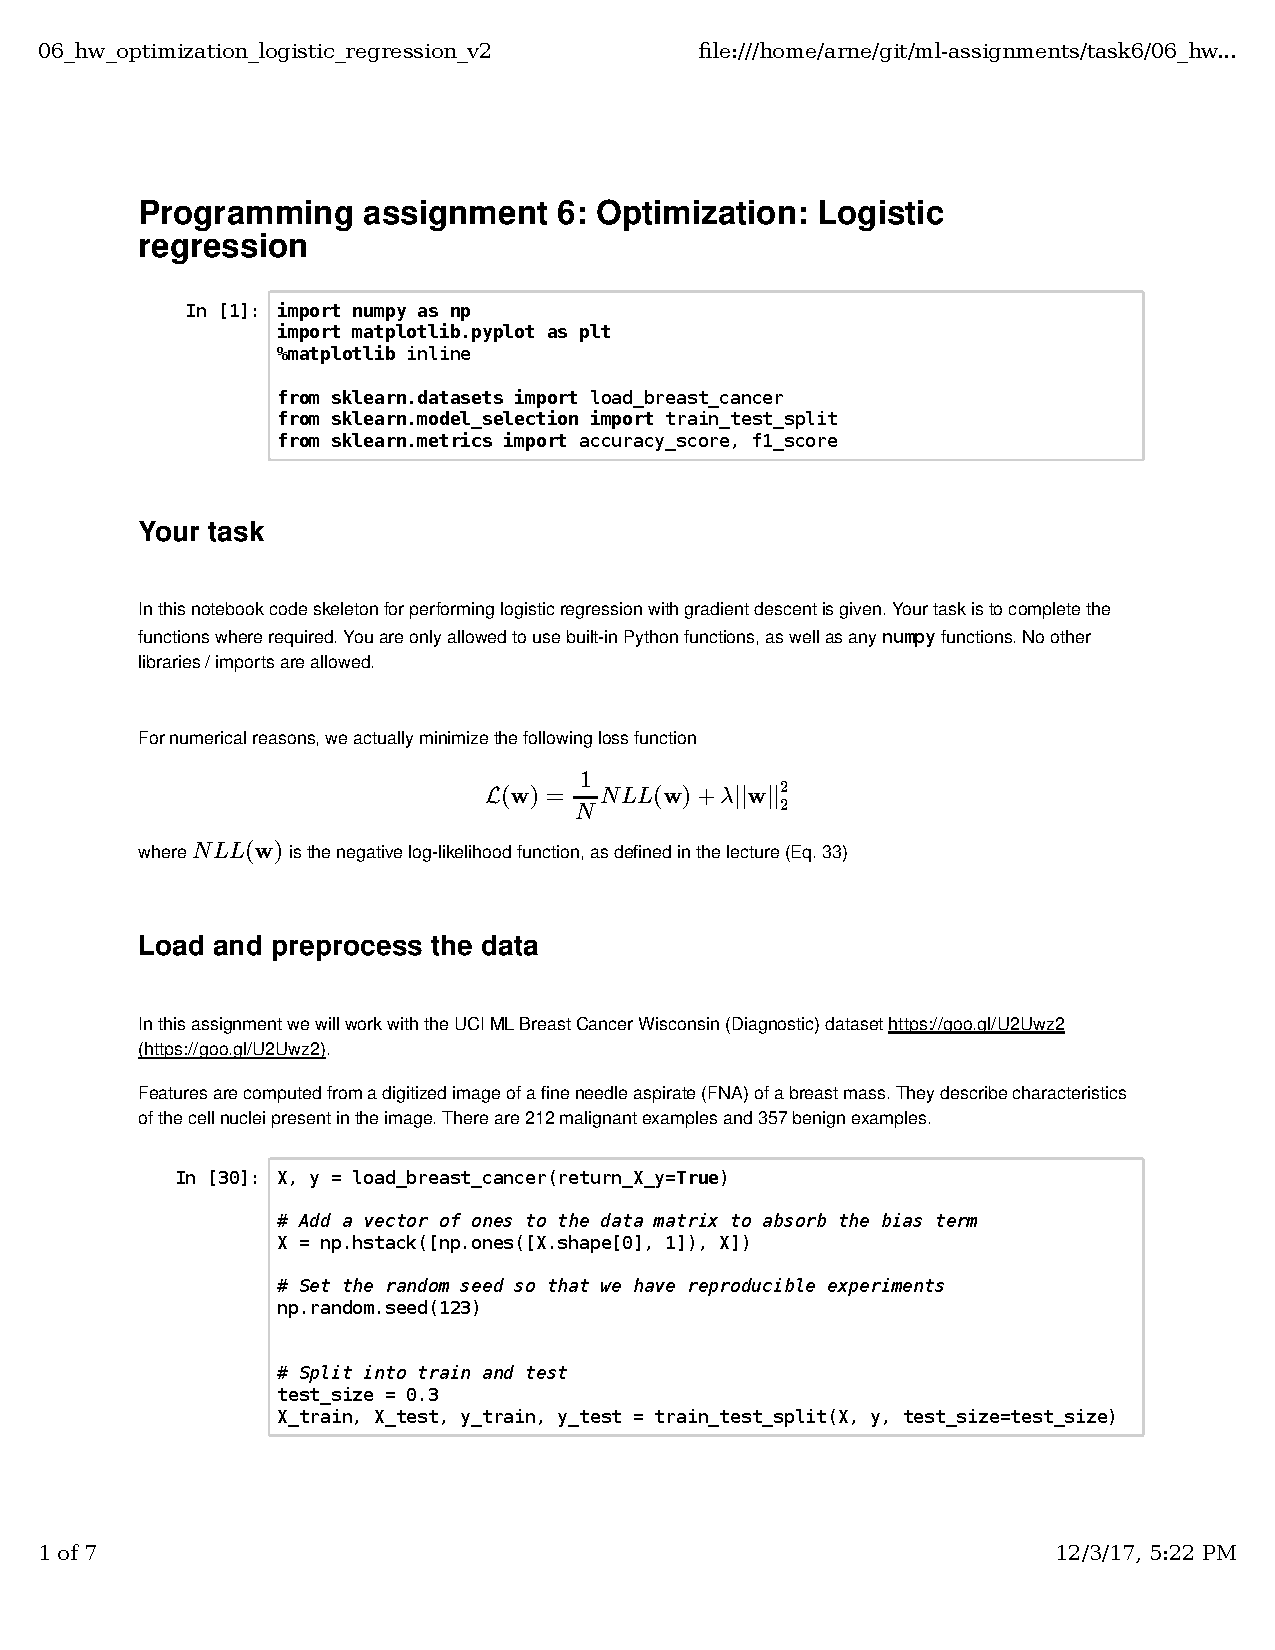
\includepdf[pages=-]{../06_hw_optimization_logistic_regression_v2}
\end{document}
